\section{Discretizing the PDE}
To maintain a bit of generality we will look at the (potentially) anisotropic diffusion equation
\begin{equation}
 \frac{\d u}{\d t} = \nabla D\nabla u +f
\end{equation}
where f is some source term. 
The final expression and scheme will depend on how we chose to approximate the time derivative, but the spatial derivative will mostly have the same approximation. \\
We start off by doing the innermost derivative in one dimension. 
The generalization to more dimesions is trivial, and will consist of adding the same terms for the y and z derivatives. 
\begin{align*}
 \left[\frac{d}{dx}u\right]^n \approx \frac{u^n_{i+1/2}-u^n_{i-1/2}}{\Delta x}
\end{align*}
Where we have made the approximate derivative around the point $x_i$. 
We then set $\phi(x)=D\frac{du}{dx}$ and do the second derivative
\begin{align*}
  \left[\frac{d}{dx}\phi\right]^n \approx \frac{\phi^n_{i+1/2}-\phi^n_{i-1/2}}{\Delta x}
\end{align*}
and insert for $\phi$
\begin{align*}
 \frac{\phi^n_{i+1/2}-\phi^n_{i-1/2}}{\Delta x} = \frac{1}{\Delta x^2}\left(D_{i+1/2}(u^n_{i+1}-u^n_{i+1}) -D_{i-1/2}(u^n_{i}-u^n_{i-1})\right)
\end{align*}
Since we can only evaluate the diffusion constant at the mesh points (or strictly speaking since it is a lot simpler to do so) we must approximate $D_{i\pm1/2}\approx0.5(D_{i\pm1}+D_i)$. 
Inerting this gives us 
\begin{equation}
 \nabla D\nabla u\approx\frac{1}{2(\Delta x+\Delta y+\Delta z)}\left((D_{i+1,j,k}+D_{i,j,k})(u_{i+1,j,k}-u_{i,j,k})-(D_{i,j,k}+D_{i-1,j,k})(u_{i,j,k}-u_{i-1,j,k})\right)
\end{equation}


\section{Some discussion}
In this numerical setup we will potentially introduce several new error sources in addition to the nomal errors introduced by numerical solution of any equation. 
When a part of the solution acquired is replaced by the solution from another model, which in this case is stochastic, we will change the initial condition to the next iteration in time. 
This might have a number of effects on our final solution. 
When we solve a differential equation numerically we only get an approximation to the actual solution because we are using approximate derivatives (see figure \ref{illustrate_approximate_derivatives}). 
We can investigate this type of error by doing two simulations of the same problem, but replacing the solution in one of the simuations in some area by the random walk model for one timestep. 

\begin{lstlisting}
 path = '/home/fredriep/Dropbox/uio/thesis/doc/results/experiment_03102013_1218/results/'
import glob

i = [];e = [];s = []

for excl in sorted(glob.glob(path+'Excl*')):
	e.append(np.load(excl))

for incl in sorted(glob.glob(path+'Incl*')):
	i.append(np.load(incl))

for j in xrange(len(i)):
	s.append(np.max(np.abs(i[j]-e[j])))
	print s[-1]
\end{lstlisting}
As we can see this will print the maximum absolute difference between the two solutions. 
Since we are dealing with a diffusion process we expect that the first timestep should have the largest error and that the error will in time be killed by the diffusion process. 
\begin{lstlisting}
[...]
0.0
0.025832
0.0054384
0.00360192
0.00212352
0.0016940416
0.0012704
0.001173512704
0.0009942699008
0.00093037021184
0.00083786862592
0.000782433954202
0.000723955260948
0.000680186522141
0.000638864266527
0.000604769629612

\end{lstlisting}
The error is larger than $\Delta t$ by a factor of $10$ ($\Delta t = 0.002$)... 
This might be improved by increasing the number of walkers, or finding a better steplength for the walkers as well as improving the walk-algorithm etc..
The above results were obtained by using the previous timestep as input to the random walk solver. 
In most numerical algorithms (Euler-Chromer etc) one will benefit from using the newest timestep as early as possible. 
Doing the same experiment with the modification of using the latest timestep as input to the random walk solver we obtain the following:
\begin{lstlisting}
[...]
0.0
0.06
0.014
0.0072
0.0036
0.00232
0.0014912
0.0011744
0.000803712
0.000703744
0.00059240448
0.000536887296
0.0004960012288
0.00047304564736
0.000437414641664
0.00041956655104
\end{lstlisting}
That is, the initial error is larger, but it is reduced faster. 
However, this is a stochastic process, and one should average over many experiments. 
An average over (only) ten experiments using twice the number of walkers (M=100) shows that the errors seem to be converging towards the same value regardless of which timestep is used as input.

\section{Manifactured Solutions}
A normal way of checking that our sceme of choise is implemented correctly is by making an exact solution to the equation and checking that the error is of the expected order. 
As a first, simple implenetation we have worked with the explicit Forward Euler discretization of the simplest form of the diffusion equation \hyperref[simple_diffusion_equation]{\ref*{simple_diffusion_equation}}. 
This discretization is expected to have an error-term of the order of $\Delta t$, which again is limited by a stability criterion. 
We can now decide that the solution to equation \ref{simple_diffusion_equation} should be
\begin{equation}\label{manifactured_solution_1D}
 u(x,t) = e^{-t\pi^2}\cos(\pi x) +1
\end{equation}
which satisfies our equation if we set the diffusion constant to 1.
\begin{align}
 \frac{\d }{\d t}e^{-t\pi^2}\cos(\pi x) +1 &= D\frac{\d^2}{\d x^2}e^{-t\pi^2}\cos(\pi x) +1\\
 -\pi^2e^{-t\pi^2}\cos(\pi x) &= -\pi^2e^{-t\pi^2}\cos(\pi x) +1 \implies 1 = 1
\end{align}
As we saw in section \ref{something_about_erroranalysis} the Forward Euler scheme is expected to have an error of the order of $\Delta t$. 
Testing only the scheme first, in 1D we get the following plot \ref{errorplot_FE1D_noWalk} of the maximum of the absolute value of the difference between the exact solution and the numerical solution to the equation. 

\begin{figure}[H]
\centering
\includegraphics[scale=0.7]{/home/fredriep/Dropbox/uio/thesis/doc/results/experiment_21102013_1141/results/errorplot.eps}
\caption{Numerical error for 1D Forwar Euler discretization.}
\label{errorplot_FE1D_noWalk}
\end{figure}

We then introduce an area on the domain where we swich models from the normal PDE to an average of the PDE solution and the result of a random walk simulation where the initial condition is the last timestep from the PDE converted to walkers by the conversion rate given in equation \ref{conversion_rate}. In this case we have used the parameters $a=3$, $\Delta t = \frac{\Delta x^2}{3.0}$, $\Delta x = \frac{1}{20}$. 
These parameters makes one unit of $u(x,t)$ equal to some $1000$ walkers. 
\begin{equation}\label{conversion_rate}
 C_{ij} = \frac{a}{\Delta t}U_{ij}
\end{equation}
The area where the model has been replaced is between $x=0.6$ and $x=0.7$, which is three mesh points. 
In the same way as for only the simple 1D PDE case we compare the combined numerical solution from the two models to the exact solution. 
Figure \ref{errorplot_FE1D_Walk_first_attemt} shows that the error is still of the order of $\Delta t$, and the difference between the two models are negligable. 
\begin{figure}[H]
\centering
\includegraphics[scale=0.7]{/home/fredriep/Dropbox/uio/thesis/doc/results/experiment_21102013_1231/results/errorplot.eps}
\caption{Numerical error for 1D Forward Euler discretization combined with random walk model between $x=0.6$ and $x=0.7$.}
\end{figure}
\subsection{2D}
Doing the same tests is 2D gives slightly different results; adding a 2D walk-domain has an influence on the error, but a rather small one. 
This can, however be tweaked by increasing the conversion parameters.